\section{The \model Architecture}\label{sec:model}


In the section, we present the \model model. 
Figure \ref{fig:model} illustrates the overall architecture. 
Given a pair of video and text input,  we design a \textbf{3D causal VAE} to compress the video into the latent space, and the latents are then patchified and unfolded into a long sequence denoted as $z_{\text{vision}}$. 
Simultaneously, we encode the textual input into text embeddings $z_{\text{text}}$ using T5~\citep{raffel2020exploring}. 
Subsequently, $z_{\text{text}}$ and $z_{\text{vision}}$ are concatenated along the sequence dimension. 
The concatenated embeddings are then fed into a stack of \textbf{expert transformer} blocks.
Finally, the model output are unpatchified to restore the original latent shape, which is then decoded using a 3D causal VAE decoder to reconstruct the video. 
We illustrate the technical design of the 3D causal VAE and expert transfomer in detail.

% \begin{wrapfigure}{l}{0.6\textwidth}
\begin{figure}[h]
\begin{center}
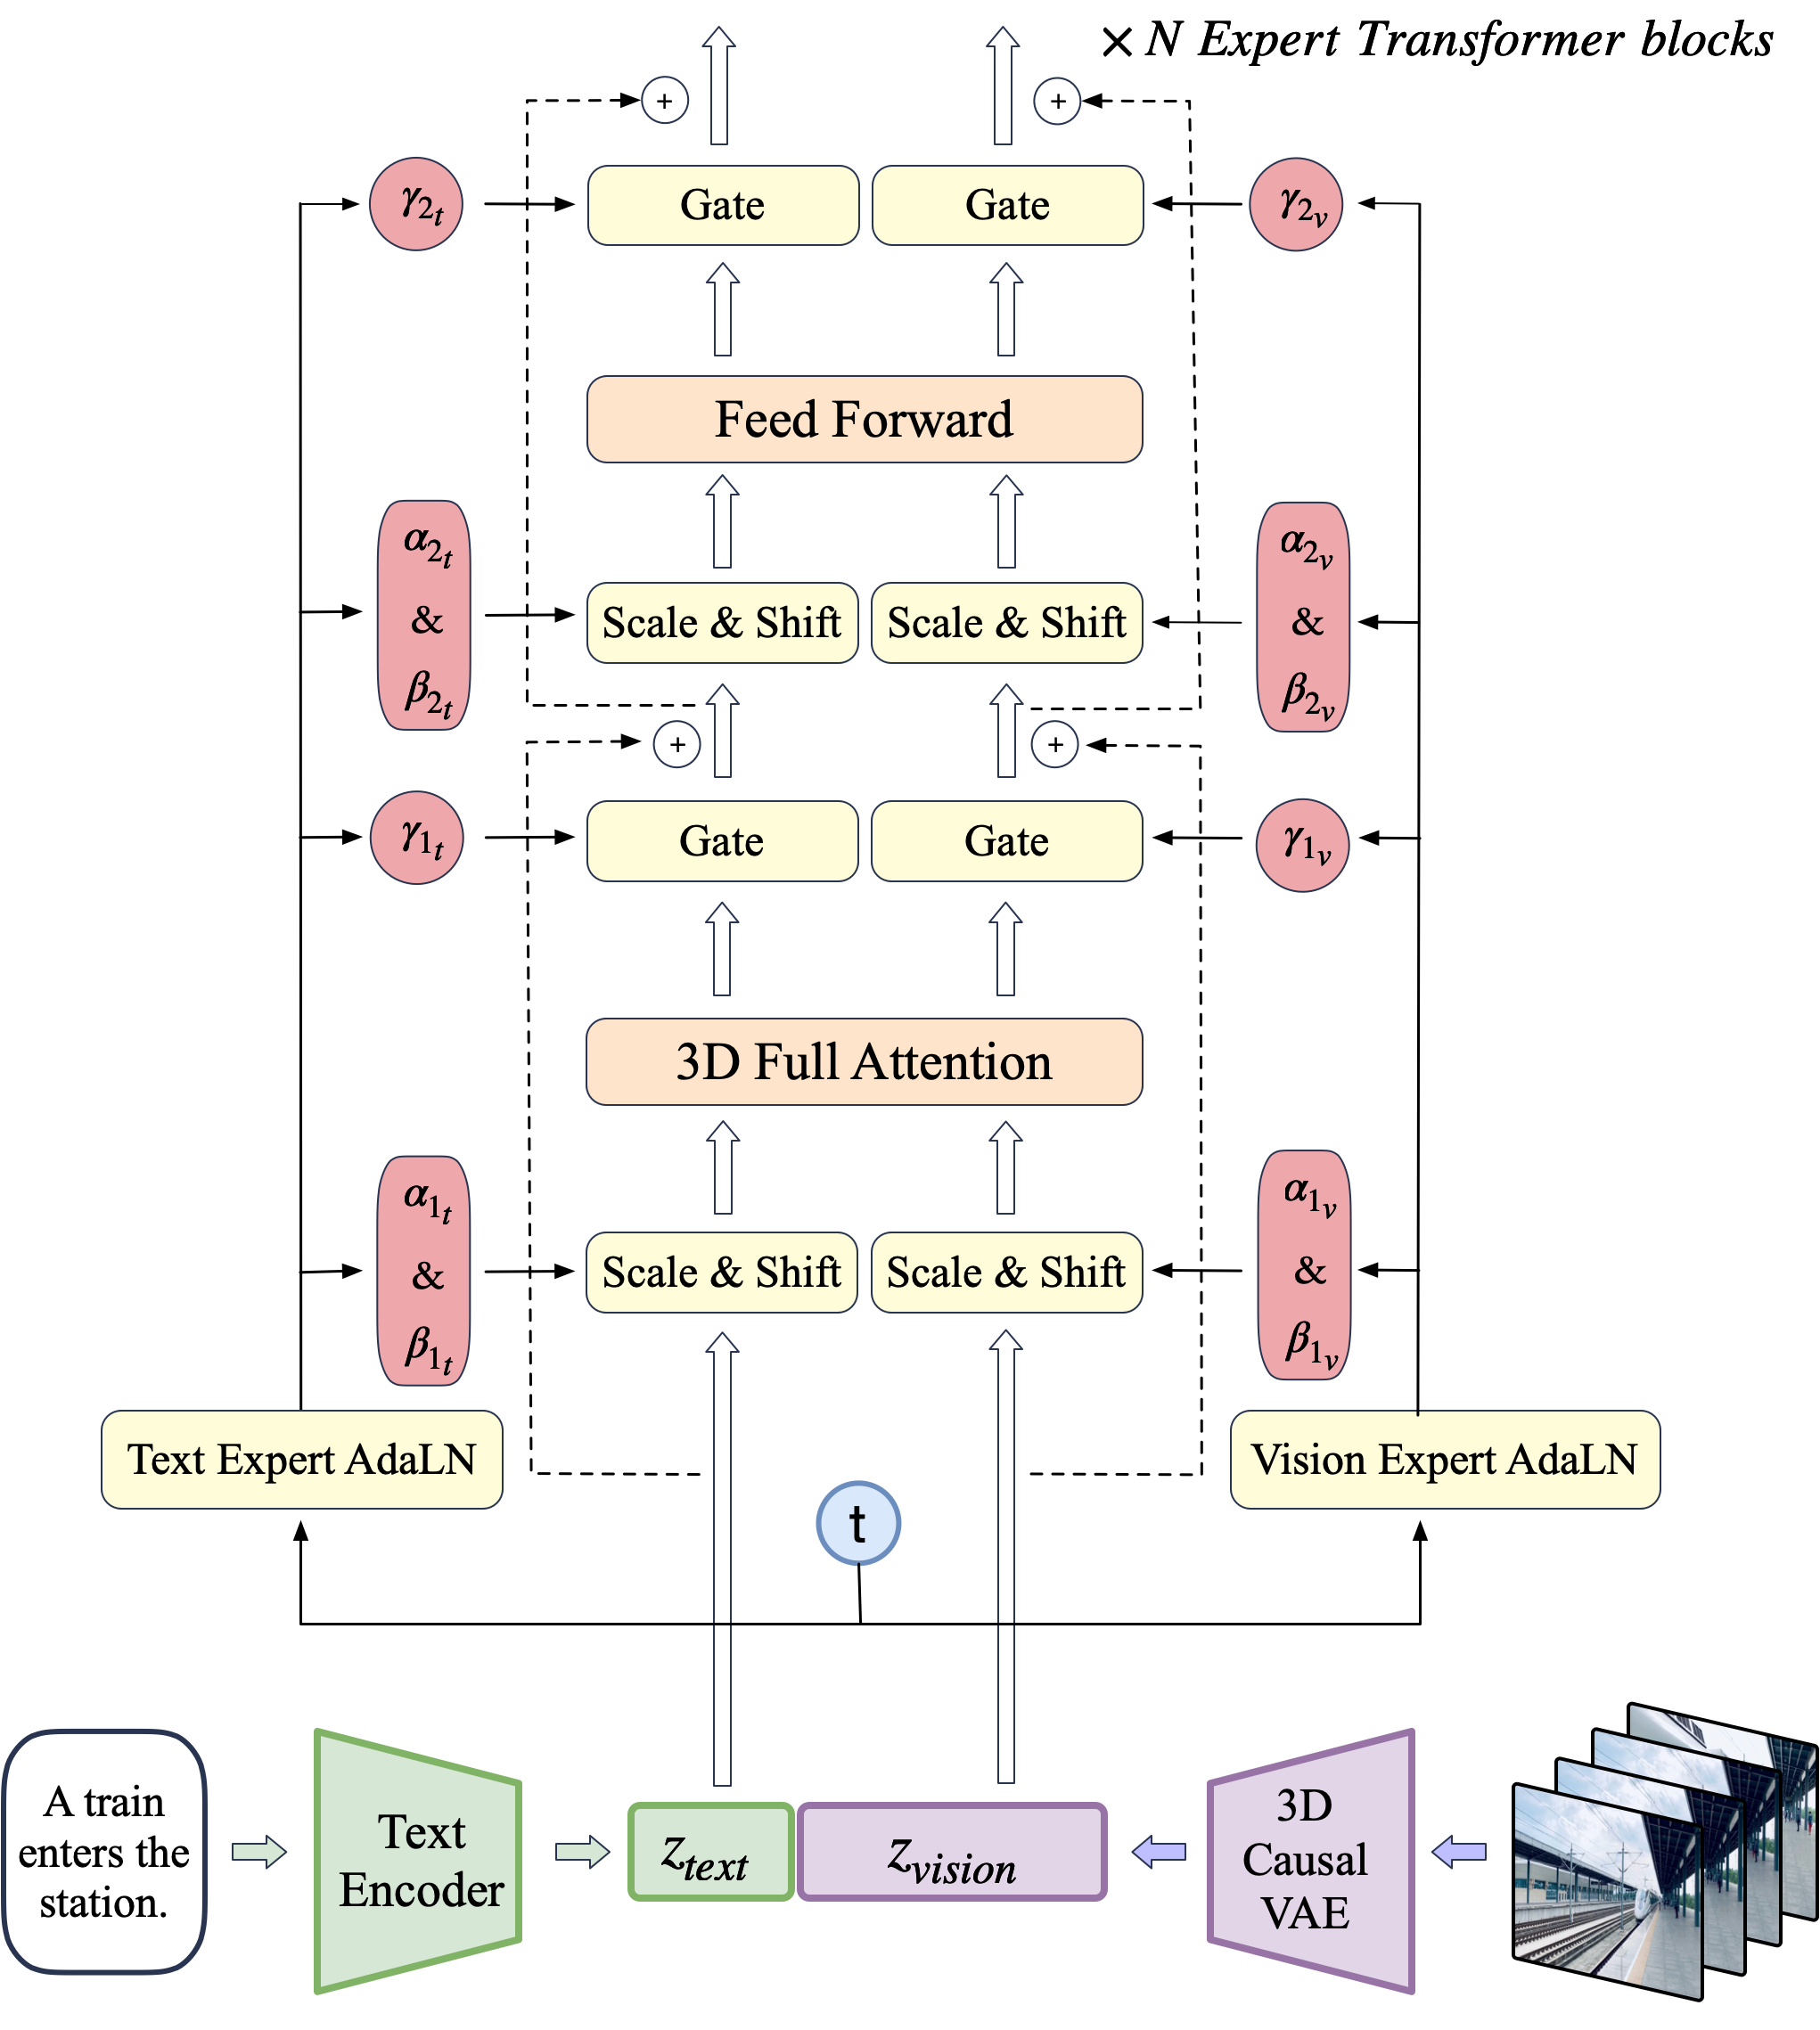
\includegraphics[width=0.6\linewidth]{images/transformer.png}
\end{center}
\caption{\textbf{The overall architecture of \model.} }
\label{fig:model}
\end{figure}
% \end{wrapfigure}



\subsection{3D Causal VAE} 

%Compared to image data, 

Videos contain both spatial and temporal information, typically resulting in much larger data volumes than images.
To tackle the computational challenge of modeling video data, we propose to implement a video compression module based on 3D Variational Autoencoders ~\citep{yu2023language}.
%Our 3D VAE
The idea is to incorporate three-dimentional convolutions to compress videos both spatially and temporally. 
This can help achieve a higher compression ratio with largely improved quality and continuity of video reconstruction.% when compared to previous image VAEs~\citep{rombach2022high, esser2021taming}. 
\begin{figure}[h]
\begin{center}
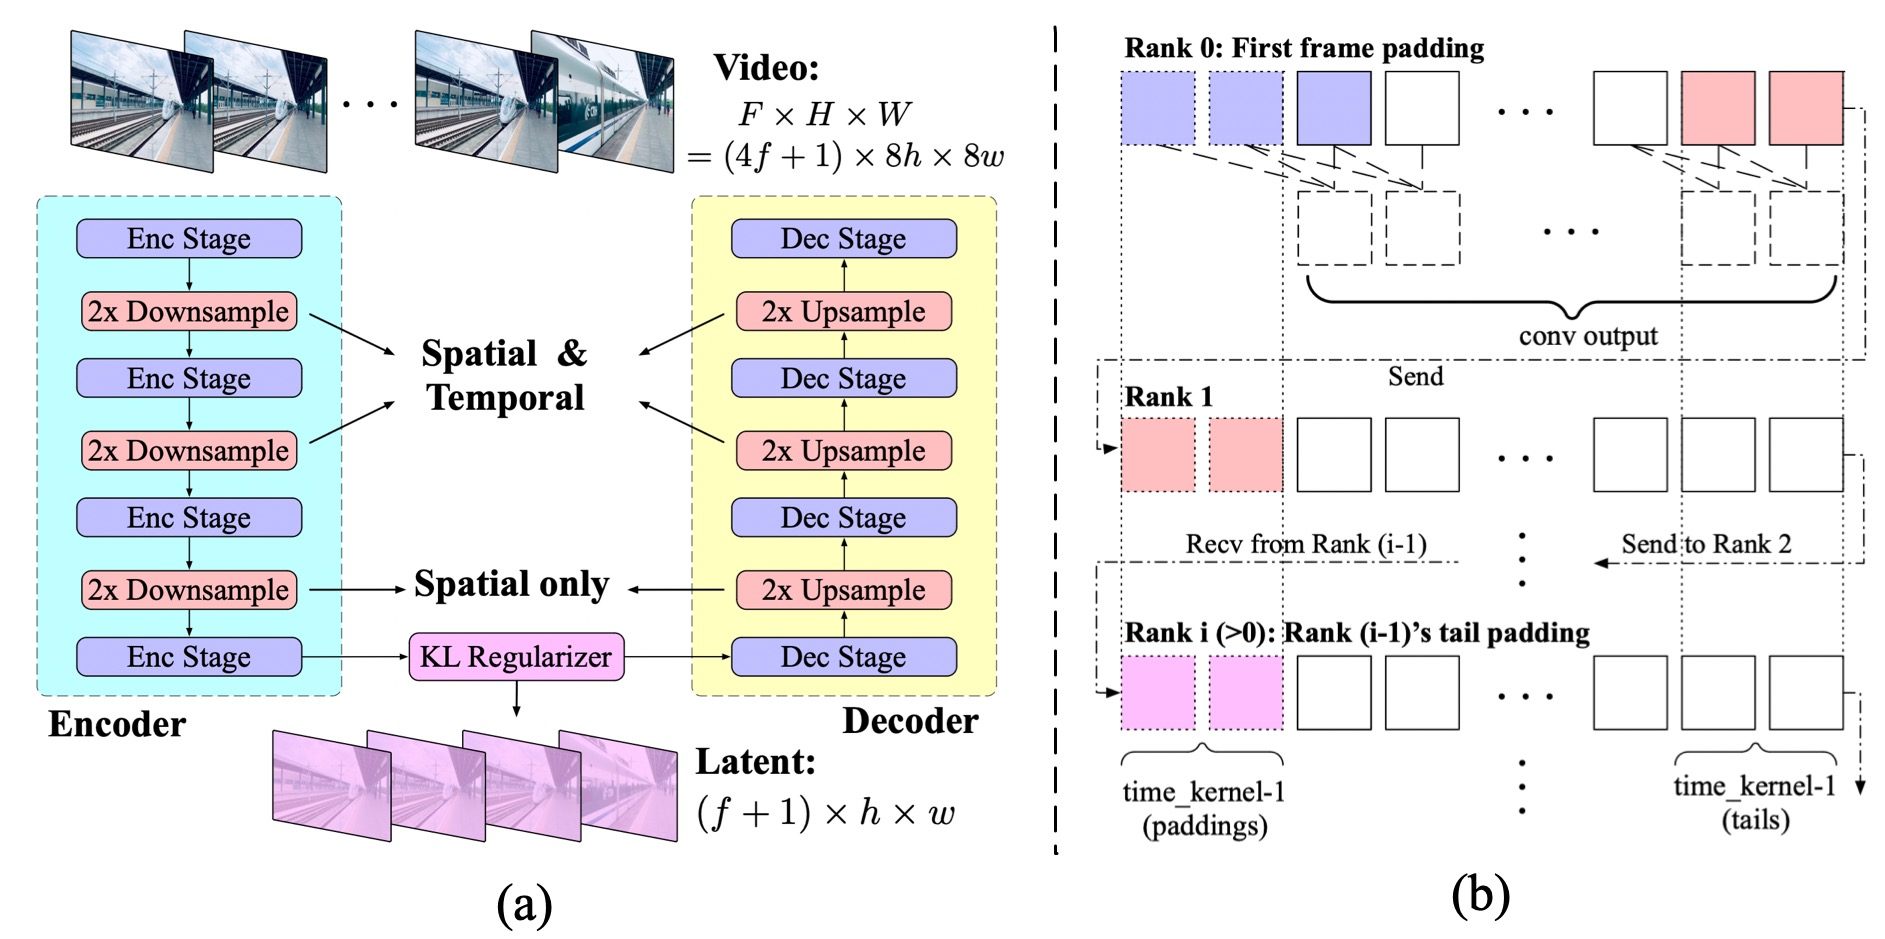
\includegraphics[width=0.8\linewidth]{images/3dvae_combined.jpg}
\end{center}
\caption{(a) The structure of the 3D VAE in \model. It comprises an encoder, a decoder and a latent space regularizer, achieving a 8$\times$8$\times$4 compression from pixels to the latents. (b) The context parallel implementation on the temporally causal convolution.}
\label{fig:3dvae_combined}
\end{figure}

Figure~\ref{fig:3dvae_combined} (a) shows the structure of the proposed 3D VAE. 
It comprises an encoder, a decoder and a latent space regularizer, Kullback-Leibler (KL) regularizer. 
% The Gaussian latent space is constrained by a Kullback-Leibler (KL) regularizer.
The encoder and decoder consist of symmetrically arranged stages, respectively performing 2$\times$ downsampling and upsampling by the interleaving of ResNet block stacked stages. Some blocks perform 3D downsampling (upsampling), while others only perform 2D downsampling (upsampling), depending on the setting.

% The first two rounds of downsampling and the last two upsampling involve both the spatial and temporal dimensions, while the last round only applies spatial sampling. 
% This enables the 3D VAE to achieve a 4$\times$ compression in the temporal dimension and an 8$\times$8 compression in the spatial dimension. 
% In total, this achieves a 4$\times$8$\times$8 spatial compression from pixels to the latents. 

We adopt the temporally causal convolution~\citep{yu2023language}, which places all the paddings at the beginning of the convolution space, as shown in Figure~\ref{fig:3dvae_combined} (b). 
This ensures that future information does not influence the present or past predictions. 

We also conducted ablation studies comparing different compression ratios and latent channels in \cref{tab:vae1}.  After using 3D structures, the reconstructed video shows almost no more jitter, and as the latent channels increase, the restoration quality improves. However, when spatial-temporal compression is too aggressive (16$\times$16$\times$8), even if the channel dimensions are correspondingly increased, the convergence of the model also becomes extremely difficult. Exploring VAE with larger compression ratios is our future work. 

\begin{table}[]
    \centering
    
    \caption{Ablation with different variants of 3D VAE. The baseline is SDXL\citep{podell2023sdxl} 2D VAE. Flickering calculates the L1 difference between each pair of adjacent frames to evaluate the degree of flickering in the video. We use variant B for pretraining.}
    \begin{tabular}{c|cccccc}
    \toprule
        Variants & Baseline & A & B & C & D & E \\ \midrule
        Compression & 8$\times$8$\times$1&8$\times$8$\times$4 & 8$\times$8$\times$4 & 8$\times$8$\times$4 & 8$\times$8$\times$8 & 16$\times$16$\times$8 \\ 
        Latent channel &4 & 8 & 16 & 32 & 32 & 128 \\ 
        Flickering$\downarrow$&93.2 & 87.6 & 86.3 & 87.7 & 87.8 & 87.3 \\ 
        PSNR$\uparrow$&28.4 & 27.2 & 28.7 & 30.5 & 29 & 27.9 \\ \bottomrule
    \end{tabular}
    \label{tab:vae1}
\end{table}



Given that processing videos with a large number of frames introduces excessive GPU memory usage, we apply context parallel at the temporal dimension for 3D convolution to distribute computation among multiple devices. 
As illustrated by Figure~\ref{fig:3dvae_combined} (b), due to the causal nature of the convolution, each rank simply sends a segment of length $k-1$ to the next rank, where $k$ indicates the temporal kernel size. 
This results in relatively low communication overhead. 
% This method can also be adapted from multi-GPU parallel to single-GPU serial processing by replacing the communication part with in-memory caching, which significantly reduces the GPU memory during inference. We call this approach \textbf{fake cp}.

During training, we first train a 3D VAE at $256\times256$ resolution and $17$ frames to save computation. Randomly select 8 or 16 fps to enhance the model's robustness.
% We observe that the encoding of larger resolution generalizes naturally, while extending the number of frames to be encoded does not work as seamlessly. 
We observe that the model can encode larger resolution videos well without additional training as it has no attention modules, but this isn't effective when encoding videos with more frames.

Therefore, we conduct a two-stage training process by first training on a video of 17 frames and finetuning by context parallel on videos of 161 frames. 
Both stages of training utilize a weighted combination of the L1 reconstruction loss, LPIPS~\citep{zhang2018unreasonable} perceptual loss, and KL loss. 
After a few thousand training steps, we introduce the GAN loss from a 3D discriminator as an additional loss term.
